%%%%%%%%%%%%%%%%%%%%%%%%%%%%%%%%%%%%%%%%%%
% Capstone Project Writeup Draft
% LaTeX Template
% Version 1.0 (November 14, 2024)
% 
% Author:
% Matías Hoyl
%
% License:
% CC BY-NC-SA 4.0 (https://creativecommons.org/licenses/by-nc-sa/4.0/)
%
%%%%%%%%%%%%%%%%%%%%%%%%%%%%%%%%%%%%%%%%%

%----------------------------------------------------------------------------------------
% PACKAGES AND OTHER DOCUMENT CONFIGURATIONS
%----------------------------------------------------------------------------------------

\documentclass[
    a4paper, % Paper size, use either a4paper or letterpaper
    10pt, % Default font size, can also use 11pt or 12pt, although this is not recommended
    % unnumberedsections, % Commented out to enable section numbering
    twoside, % Two side traditional mode where headers and footers change between odd and even pages, comment this option to make them fixed
]{LTJournalArticle}

\usepackage{indentfirst} % Add this line to indent the first paragraph of each section

\usepackage{tabularx}

\addbibresource{references.bib} % BibLaTeX bibliography file

\runninghead{Synthetic Students} % Updated running head

\setcounter{page}{1} % The page number of the first page, set this to a higher number if the article is to be part of an issue or larger work

\usepackage{tcolorbox}
\tcbuselibrary{breakable, skins}

\usepackage{xcolor}

\usepackage{float} % Add this line to include the float package

\usepackage{enumitem} % Ensure this package is included

% Explicitly set spacing for enumerate environments
\setlist[enumerate]{noitemsep, topsep=0pt, partopsep=4pt, parsep=4pt}

% Define slate color palette
\definecolor{slate-50}{HTML}{F8FAFC}
\definecolor{slate-100}{HTML}{F1F5F9}
\definecolor{slate-200}{HTML}{E2E8F0}
\definecolor{slate-300}{HTML}{CBD5E1}
\definecolor{slate-400}{HTML}{94A3B8}
\definecolor{slate-500}{HTML}{64748B}
\definecolor{slate-600}{HTML}{475569}
\definecolor{slate-700}{HTML}{334155}
\definecolor{slate-800}{HTML}{1E293B}
\definecolor{slate-900}{HTML}{0F172A}

% Then use the tcolorbox definition as before
\newtcolorbox{promptbox}{
    colback=slate-100,
    colframe=slate-400,
    boxrule=0.5pt,
    arc=2pt,
    fontupper=\ttfamily\footnotesize,
    left=10pt,
    right=10pt,
    top=8pt,
    bottom=8pt,
    breakable
}

% First make sure you have the correct tcolorbox libraries loaded
\usepackage{tcolorbox}
\tcbuselibrary{breakable,skins}

% Define slate color palette (keep your existing color definitions)
\definecolor{slate-50}{HTML}{F8FAFC}
\definecolor{slate-100}{HTML}{F1F5F9}
\definecolor{slate-200}{HTML}{E2E8F0}
\definecolor{slate-300}{HTML}{CBD5E1}
\definecolor{slate-400}{HTML}{94A3B8}
\definecolor{slate-500}{HTML}{64748B}
\definecolor{slate-600}{HTML}{475569}
\definecolor{slate-700}{HTML}{334155}
\definecolor{slate-800}{HTML}{1E293B}
\definecolor{slate-900}{HTML}{0F172A}

% Updated box definitions
\newtcolorbox{questionbox}[2][]{%
    enhanced,
    colback=slate-50,
    colframe=slate-400,
    boxrule=0.5pt,
    arc=4pt,
    title={#2},
    fonttitle=\bfseries\color{white},
    attach boxed title to top left={xshift=0.5cm,yshift=-\tcboxedtitleheight/2},
    boxed title style={
        colback=slate-400,
        colframe=slate-400,
        arc=2pt,
        boxrule=0pt,
    },
    top=12pt, % Increased top padding
    breakable,
    #1
}

\newtcolorbox{studentbox}[2][]{%
    enhanced,
    colback=slate-100,
    colframe=slate-500,
    boxrule=0.5pt,
    arc=4pt,
    title={#2},
    fonttitle=\bfseries\color{white},
    attach boxed title to top left={xshift=0.5cm,yshift=-\tcboxedtitleheight/2},
    boxed title style={
        colback=slate-500,
        colframe=slate-500,
        arc=2pt,
        boxrule=0pt,
    },
    top=12pt,
    breakable,
    #1
}

\newtcolorbox{llmbox}[2][]{%
    enhanced,
    colback=slate-200,
    colframe=slate-600,
    boxrule=0.5pt,
    arc=4pt,
    title={#2},
    fonttitle=\bfseries\color{white},
    attach boxed title to top left={xshift=0.5cm,yshift=-\tcboxedtitleheight/2},
    boxed title style={
        colback=slate-600,
        colframe=slate-600,
        arc=2pt,
        boxrule=0pt,
    },
    top=12pt,
    breakable,
    #1
}

%----------------------------------------------------------------------------------------
% TITLE SECTION
%----------------------------------------------------------------------------------------

\title{Synthetic Students: Using Item Response Theory to Guide LLM-Based Answer Prediction} 

% Authors are listed in a comma-separated list with superscript numbers indicating affiliations
% \thanks{} is used for any text that should be placed in a footnote on the first page, such as the corresponding author's email, journal acceptance dates, a copyright/license notice, keywords, etc
\author{% 
    Matías Hoyl\textsuperscript{1} 
}

% Affiliations are output in the \date{} command
\date{\footnotesize \textsuperscript{1}School of Education, Stanford University}

\begin{document}

\maketitle

%----------------------------------------------------------------------------------------
% SECTION: INTRODUCTION
%----------------------------------------------------------------------------------------
\section{Introduction}

Educational assessment faces two key challenges: developing high-quality test items is expensive, and calibrating these items requires extensive student data. This paper explores a potential solution by combining Item Response Theory (IRT) with Large Language Models (LLMs) to create "synthetic students" - AI systems that can simulate how real students would respond to test questions.

Traditional IRT methods use statistical models to measure student abilities and question difficulty. LLMs, meanwhile, have shown impressive capabilities in understanding and generating human-like text. By combining these approaches, we aim to create a system that can predict student responses accurately enough to help with initial item calibration, potentially reducing the need for extensive field testing.

Our research uses data from Zapien, an educational technology platform, with over 280,000 student interactions on mathematics questions. We investigate two fundamental questions:

\begin{enumerate}
    \item Can LLMs effectively simulate student response patterns when given information about student abilities and question characteristics?
    \item What contextual information (such as prior performance, topic mastery, or demographic data) most effectively guides LLMs to generate realistic student responses?
\end{enumerate}

Our preliminary results show that LLMs can improve upon baseline simulations of student responses when provided with detailed context about student ability and prior performance. However, additional research is needed to validate these findings and determine their practical significance. With further development, synthetic students may help streamline aspects of the test development process while maintaining assessment quality.

This research offers a practical approach to improving educational assessment development, combining the statistical rigor of psychometrics with recent advances in artificial intelligence.

%----------------------------------------------------------------------------------------
% SECTION: RELATED WORK
%----------------------------------------------------------------------------------------
\section{Related Work}

\subsection{Enhancing IRT Models}
Item Response Theory (IRT) has long been a foundational method for modeling student performance and estimating item characteristics, yet it often relies solely on item response data. Recent research has highlighted the potential to enhance IRT models by incorporating additional collateral information, such as examinee demographics or item features, to improve the estimation of item parameters and student abilities.

\textcite{mislevy1988collateral} explored the use of collateral information in the estimation of item parameters within IRT models, arguing that the inclusion of additional data beyond item responses can enhance the precision and reliability of parameter estimates. This study used Bayesian statistical modeling techniques to integrate supplementary information, such as item content and cognitive processing requirements, as well as examinee demographics like educational background. By exploiting this collateral information, IRT models can provide more nuanced insights into both item difficulty and individual student abilities, allowing for a richer and more context-sensitive understanding of learning outcomes.

Building on this concept, \textcite{thomas2002complex} examined the application of IRT methods to complex survey data, such as those collected in the National Longitudinal Survey for Children and Youth (NLSCY). They demonstrated that while IRT is well-suited for evaluating abilities within diverse populations, issues like bias can arise if survey-specific features, such as weights and clustering, are ignored. The study underscored the importance of addressing these biases by incorporating survey weights and other structural elements into IRT modeling, which can lead to more accurate and representative estimates of student ability. This approach shows that extending IRT to accommodate complex data structures can significantly enhance its utility in educational research, particularly when dealing with heterogeneous populations.

These studies collectively emphasize that the effectiveness of IRT models can be improved by leveraging additional contextual information. By incorporating details about item formats, examinee backgrounds, and survey-specific characteristics, educators and researchers can achieve a deeper and more precise understanding of both student performance and item characteristics, ultimately leading to more effective adaptive learning systems.

\subsection{LLMs in Assessment Generation and Grading}
Large Language Models (LLMs) have transformed educational assessment automation. \textcite{fagbohun2024beyond} showed that LLMs can grade both short answers and essays effectively, providing detailed feedback that addresses common limitations of traditional grading. A comprehensive systematic review by \textcite{gao2023automatic} analyzed 93 studies on automated assessment systems in higher education, confirming that modern LLMs can evaluate open-ended responses with high accuracy. Their review emphasized how AI-powered tools have evolved to handle increasingly complex student responses while maintaining consistent evaluation standards.

LLMs also show significant promise in creating assessment materials. In medical education, \textcite{artsi2024large} conducted a systematic review of LLM applications in exam generation. While LLMs can produce multiple-choice questions efficiently, the study found that outputs require expert review to meet professional standards. This limitation highlights the current role of LLMs as assistive tools rather than complete replacements for expert test developers.

In K-12 education, \textcite{zelikman2023generating} made significant advances in automated test creation. Their system generated reading assessment tests that achieved high correlation (r=0.93) with expert-written versions. The study combined LLM-based item generation with sophisticated simulation techniques to evaluate question difficulty and ambiguity automatically. This approach offers a scalable method for creating parallel test forms while maintaining quality standards.

\subsection{LLMs in Student Behavior Simulation} 
Recent research has demonstrated LLMs' ability to accurately simulate human behavior patterns. \textcite{argyle2022out} showed that LLMs can generate realistic "silicon samples" when properly conditioned on demographic data. Their work introduced the concept of "algorithmic fidelity" - the ability of LLMs to capture and reproduce complex patterns of human responses. Building on this foundation, \textcite{park2023generative} developed more sophisticated "generative agents" by incorporating memory streams, reflection mechanisms, and planning capabilities. These additions allowed for more authentic and dynamic behavioral simulations.

In educational contexts, \textcite{xu2023leveraging} demonstrated that LLMs can effectively simulate student learning behaviors by modeling relationships between prior knowledge, engagement levels, and understanding. Their research showed that simulation accuracy improved significantly when incorporating detailed student assessment history. This finding suggests that rich historical data is crucial for creating realistic student models.

\textcite{lu2024generative} further advanced this field with their "Generative Students" framework, achieving strong correlation between simulated and real student responses on multiple-choice assessments. Their approach focused on modeling student profiles based on mastery levels, confusion patterns, and knowledge gaps. The framework proved particularly effective at identifying which questions would challenge actual students, demonstrating its value for test development and validation.

These advances in both assessment automation and behavior simulation suggest complementary roles for LLMs in education. Assessment tools can provide efficient, consistent evaluation at scale, while simulation capabilities help understand and predict student behavior patterns. However, both applications currently require human oversight to ensure validity and appropriate implementation. Future research may focus on integrating these capabilities to create more adaptive and responsive educational systems.

\subsection{Gaps in Current Research}

While Item Response Theory (IRT) has significantly benefited from the inclusion of additional contextual information, such as demographic or item features, these enhancements remain relatively restricted and parameterized. The current use of collateral data in IRT is often constrained to predetermined factors that limit the model's flexibility. Despite the improvements in accuracy, these models are still rigid in adapting to the complexity and variability of individual student responses, especially in dynamically changing learning environments.

Conversely, Large Language Models (LLMs) have been extensively used for educational purposes, particularly in generating teacher-centric content, such as lesson plans, assessments, and grading rubrics. On the learner side, LLMs have been deployed effectively as tutors, simulating learning scenarios and providing personalized feedback. However, their application in directly simulating student responses remains relatively underdeveloped. Most work to date focuses on utilizing LLMs for generating instructional content or guiding student learning, rather than capturing the nuance and unpredictability of student responses.

One promising yet unexplored avenue is the simulation of student responses by leveraging the flexibility and adaptiveness of LLMs in conjunction with the strong predictive signals provided by IRT parameters. Such a hybrid approach could take advantage of IRT's robust psychometric foundation while utilizing LLMs' nuanced understanding of language and context to simulate realistic student behaviors, including mistakes, reasoning patterns, and hesitation.

If successful, this research could improve the calibration of educational items. Synthetic students powered by LLMs could be used to conduct an initial round of item calibration, offering a cost-effective and faster alternative to traditional methods, which require extensive testing with actual students. By first passing items through these synthetic agents, preliminary item parameters could be established and refined through real student interactions, thereby optimizing the calibration process and reducing the need for costly, large-scale field testing. This would lead to more efficient and adaptive learning systems, capable of adjusting to diverse educational contexts while maintaining psychometric standards.

%----------------------------------------------------------------------------------------
% SECTION: DATA
%----------------------------------------------------------------------------------------
\section{Data}

\subsection{Overview}
The dataset used in this study originates from Zapien, an adaptive educational technology platform based in Chile, focused on helping students learn mathematics. The dataset contains 280,979 answers from approximately 5,000 students across 50+ schools. Each record represents an interaction between a student and the platform, providing information on the student's skill level, question attributes, and outcomes.

Key features of the dataset include:
\begin{itemize}
    \item Student demographic information and skill levels
    \item Question characteristics (options, text) and difficulty metrics
    \item Response data including correctness and timing
    \item Topic and subject categorization
    \item School and grade-level information
\end{itemize}

\subsection{Data Preprocessing}
Data preprocessing involved several key steps to ensure data quality:
\begin{itemize}
    \item Removal of rows with missing values on key variables, like \texttt{use\_level}, \texttt{question\_id}, \texttt{correct}, and \texttt{time\_taken}
    \item Filtering out students with fewer than 20 questions answered, as their \texttt{user\_level} metric has not yet converged to a true value
    \item Removing observations with \texttt{difficulty} or \texttt{user\_level} values outside the -3 to 3 range
    \item Excluding responses with unrealistic timing (less than 3 seconds, likely due to random guessing, or greater than 10 minutes, probably outliers who left the platform)
\end{itemize}

The dataset was split into an 80-20 training and holdout set, with 224,783 rows allocated for analysis and 56,196 reserved for evaluation on unseen students.

\subsection{Feature Engineering}
The following features were engineered to provide richer context for the LLM simulations:

\begin{itemize}
    \item \texttt{student\_time\_taken}: Calculated based on timestamps to represent the time each student took to answer questions
    \item \texttt{avg\_question\_time}: Average response time for each question across all students
    \item \texttt{student\_attempts} and \texttt{student\_correct}: Cumulative counters for each student, capturing attempts and correctness at multiple granularity levels (e.g., question, topic)
\end{itemize}

\subsection{Data Exploration}
Key variables are analyzed to understand their distributions and identify patterns in student behavior.

\subsubsection{Univariate Analysis}
Individual variable distributions are examined to assess data quality and baseline characteristics.

\paragraph{Distribution of Student Time Taken}
Most students answer within 3-20 seconds, with some taking longer due to question complexity or individual differences.

\begin{figure}[H]
    \centering
    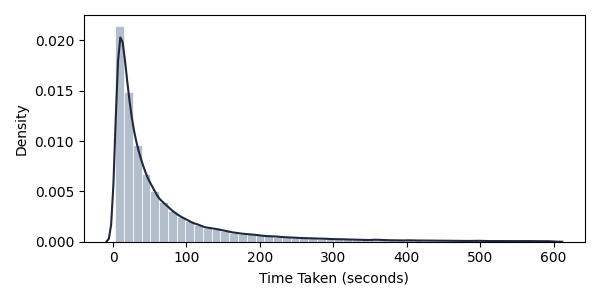
\includegraphics[width=\columnwidth]{images/time_distribution.png}
    \caption{Distribution of Time Taken by Students}
    \label{fig:time-distribution}
\end{figure}

\paragraph{Distribution of Correctness}
The questions seem to be unbalanced, with approximately 70\% correct and 30\% incorrect answers.

\begin{figure}[H]
    \centering
    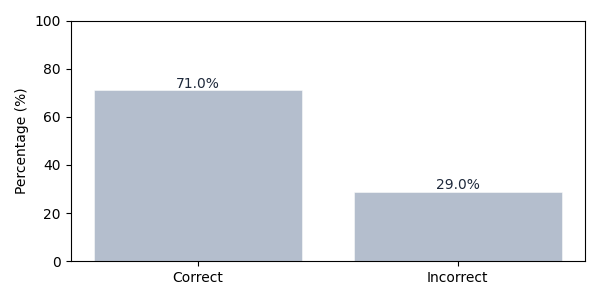
\includegraphics[width=\columnwidth]{images/correct_incorrect_dist.png}
    \caption{Proportion of Correct and Incorrect Answers}
    \label{fig:correct-incorrect-dist}
\end{figure}

\paragraph{Distribution of User Level}
The distribution of user levels follows a roughly normal distribution centered around -1.5, with a notable spike at the lowest skill level. This suggests a diverse range of abilities among students, with a significant number of beginners or struggling users.

\begin{figure}[H]
    \centering
    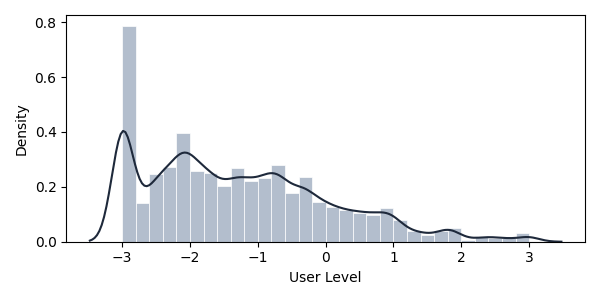
\includegraphics[width=\columnwidth]{images/user_level_dist.png}
    \caption{Distribution of Latest User Levels}
    \label{fig:user-level-dist}
\end{figure}

\paragraph{Distribution of Average Question Time}
The distribution of average question time appears to follow a skewed normal distribution centered around 50 seconds, with a long right tail. This indicates that while most questions are answered within a reasonable timeframe, some questions may require more time, possibly due to higher complexity or ambiguity.

\begin{figure}[H]
    \centering
    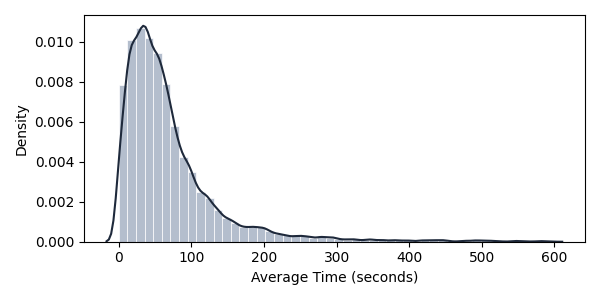
\includegraphics[width=\columnwidth]{images/avg_time_distribution.png}
    \caption{Distribution of Average Question Time}
    \label{fig:avg-time-dist}
\end{figure}

\paragraph{Distribution of Question Success Ratio}
There is a high concentration of questions with a success ratio of 1.0, indicating many students achieve perfect scores on certain questions. This could reflect well-designed questions that effectively assess student knowledge, but it also suggests the need for more challenging questions to better differentiate student abilities.

\begin{figure}[H]
    \centering
    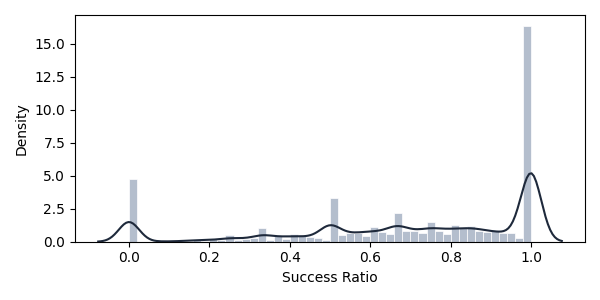
\includegraphics[width=\columnwidth]{images/success_ratio_distribution.png}
    \caption{Distribution of Question Success Ratio}
    \label{fig:success-ratio-dist}
\end{figure}

\paragraph{Distribution of Question Difficulty}
The distribution of difficulty is bounded between -3 and 3, with notable spikes at integer values, suggesting the use of rounding functions that prioritize integer numbers. 

\begin{figure}[H]
    \centering
    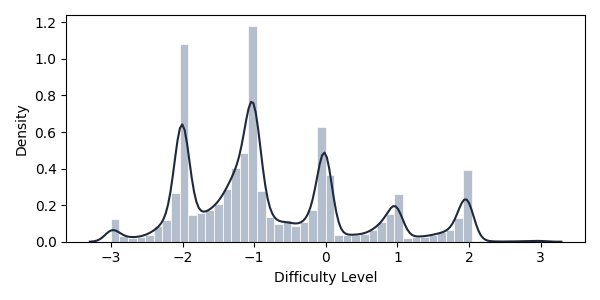
\includegraphics[width=\columnwidth]{images/difficulty_distribution.png}
    \caption{Distribution of Question Difficulty}
    \label{fig:difficulty-dist}
\end{figure}

\subsubsection{Bivariate Analysis}
We analyze relationships between variables to identify patterns and correlations, crucial for simulating student behavior.
% Remove any potential blank lines here
\paragraph{Student Time Taken vs. Correctness}
Students who answered incorrectly took slightly longer on average than those who answered correctly. This pattern could be due to incorrect answers coming from more challenging questions that require more time, or due to a high concentration of easily answerable questions in the dataset.

\begin{figure}[H]
    \centering
    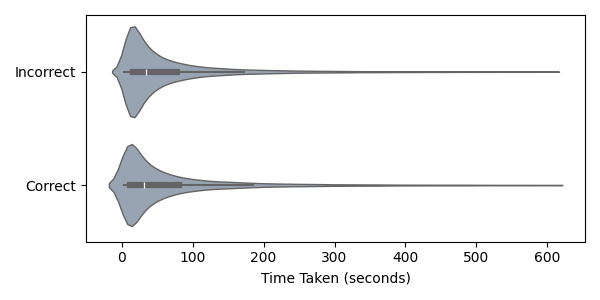
\includegraphics[width=\columnwidth]{images/time_vs_correctness.png}
    \caption{Time Taken vs. Correctness}
    \label{fig:time-vs-correctness}
\end{figure}

\paragraph{Avg Question Time vs. Correctness}
Questions that students answered correctly tend to have longer average completion times. This pattern shows a correlation between time spent and correctness.
\begin{figure}[H]
    \centering
    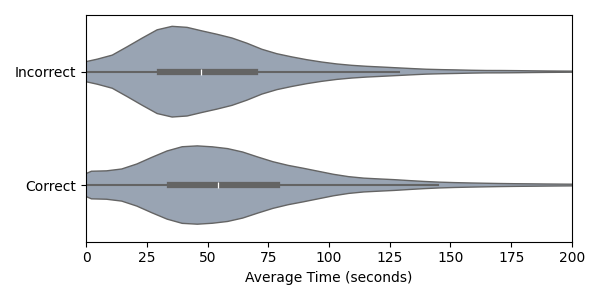
\includegraphics[width=\columnwidth]{images/avg_time_vs_correctness.png}
    \caption{Average Question Time vs. Correctness}
    \label{fig:avg-time-vs-correctness}
\end{figure}

\paragraph{Difficulty vs. Correctness}
The data shows a high concentration of questions in the lower difficulty range, suggesting a tendency towards easier questions. Despite this skew towards lower difficulty, there are no substantial differences in correctness rates across difficulty levels, indicating that the difficulty metric may not be effectively discriminating between question complexity.
\begin{figure}[H]
    \centering
    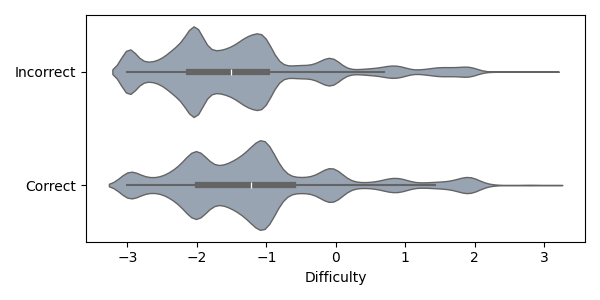
\includegraphics[width=\columnwidth]{images/difficulty_vs_correctness.png}
    \caption{Question Difficulty vs. Correctness}
    \label{fig:difficulty-vs-correctness}
\end{figure}

\paragraph{User Level vs. Correctness}
Lower user levels correlate with higher correctness rates. This inverse relationship likely stems from the platform's adaptive behavior, where students with lower levels are presented with easier questions, resulting in a higher concentration of correct answers. This suggests the platform effectively adjusts question difficulty based on user level to maintain engagement and success.
\begin{figure}[H]
    \centering
    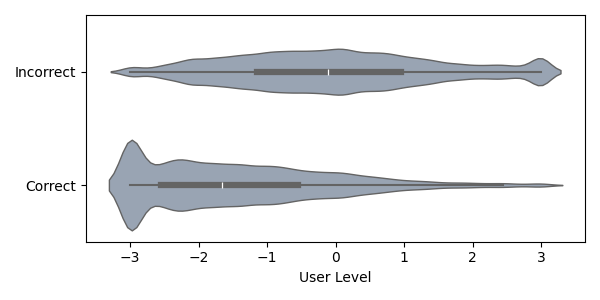
\includegraphics[width=\columnwidth]{images/user_level_vs_correctness.png}
    \caption{User Level vs. Correctness}
    \label{fig:user-level-vs-correctness}
\end{figure}

\paragraph{Question Success Ratio vs. Difficulty}
There is a negative correlation between question difficulty and success rate. This relationship highlights the importance of balancing question difficulty to maintain student engagement and accurately assess their abilities.

\begin{figure}[H]
    \centering
    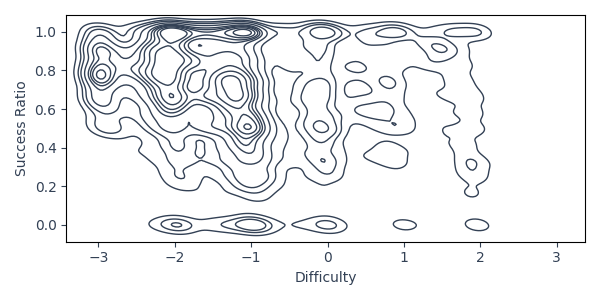
\includegraphics[width=\columnwidth]{images/success_ratio_vs_difficulty_kde.png}
    \caption{Question Success Ratio vs. Difficulty}
    \label{fig:success-ratio-vs-difficulty}
\end{figure}

\subsubsection{Multivariate Analysis}
We explore relationships between multiple variables to identify patterns and correlations. This analysis helps in understanding the complex interactions that can influence student performance.

\paragraph{Heatmap of Correlation Matrix}
The heatmap shows that user level has positive correlations with correct answers and question success ratio, indicating better performance from experienced users. It also reveals that higher-level users tend to receive more difficult questions. Question difficulty shows expected negative correlations with success rates, while time metrics demonstrate consistency in time spent across questions.

\begin{figure}[H]
    \centering
    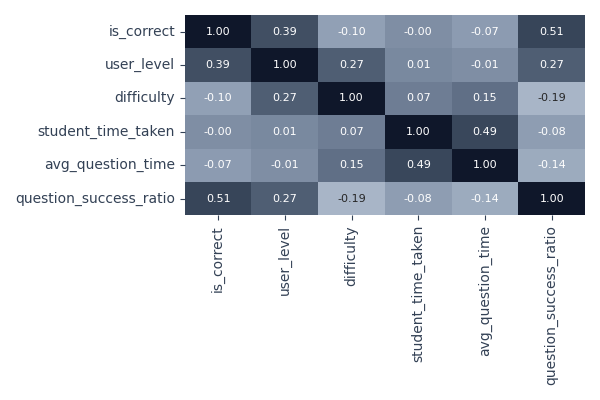
\includegraphics[width=\columnwidth]{images/correlation_matrix.png}
    \caption{Correlation Matrix}
    \label{fig:correlation-matrix}
\end{figure}



%----------------------------------------------------------------------------------------
% SECTION: METHODS
%----------------------------------------------------------------------------------------
\section{Methods}

\subsection{Simulation Approach}
In this study, we used Large Language Models (LLMs) to simulate student responses to mathematics questions under varying conditions. Our approach consisted of multiple experimental scenarios designed to evaluate how well LLMs can predict student responses when provided with different levels of contextual information.

\subsubsection{Baseline Scenario}
In the baseline scenario, the LLMs were provided with minimal context, specifically the student's age and grade level. This served as a control to determine how well LLMs could respond to mathematics questions with limited information, without much insight into the student's skill or history.

The baseline prompt was structured as follows:

\begin{promptbox}
    \#\#\# Begin Role \#\#\#
    
    You are simulating a student taking a mathematics assessment. Your role is to authentically embody a student and answer a question how the student would.
    
    Remember that you are not an AI, but rather a student with human characteristics, including occasional self-doubt, varying motivation levels, and the potential to make mistakes that align with your profile.
    
    \#\#\# End Role \#\#\#
    
    \vspace{1em}
    
    \#\#\# Begin Student Profile \#\#\#
    
    You are \{\{studentAge\}\} years old
    
    \#\#\# End Student Profile \#\#\#

    \vspace{1em}
    
    \#\#\# Begin Question Context \#\#\#
    
    You are now facing a question with these characteristics:
    
    - Topic: \{\{topicName\}\}
    
    - Subject: \{\{subjectName\}\}
    
    - Axis: \{\{axisName\}\}
    
    - Question:
    
    \{\{question\}\}
    
    - Options:
    
    (a) \{\{optionA\}\}
    
    (b) \{\{optionB\}\}
    
    (c) \{\{optionC\}\}
    
    (d) \{\{optionD\}\}
    
    (e) \{\{optionE\}\}
    
    \#\#\# End Question Context \#\#\#

    \vspace{1em}
    
    \#\#\# Begin Instructions \#\#\#
    
    Read the question.
    
    Think through the problem as a student would:
    
    - Consider what parts you understand
    
    - Note what might confuse you
    
    - Think about similar problems you might have seen before
    
    \#\#\# End Instructions \#\#\#

    \vspace{1em}
    
    \#\#\# Begin Response Format \#\#\#
    
    Your response MUST be formatted as JSON with the following structure:
    
    \{
    
        "response": \{
    
            "thinking": "Here goes your thinking process. You should write a few sentences describing your initial thoughts about the problem, how you would approach it, and any potential pitfalls you might encounter. Finally, you should mention your final choice and some rationale around why you chose it.",
    
            "answer": "Your final choice. Between these two tags, you should only write one lower-case letter (a, b, c, d or e). Nothing more, so that I can parse it easily.",
    
            "confidence": "How sure you are about your answer. A number between 0 and 100. Only the number, no other characters, so that I can parse it easily. This should be a number, not a string."
    
        \}
    
    \}
    
    \#\#\# End Response Format \#\#\#

    \vspace{1em}
    
    \#\#\# Begin Important Reminder \#\#\#
    
    Remember, you are simulating a student. Don't just write the correct answer, but try to simulate what a student would do.
    
    \#\#\# End Important Reminder \#\#\#
\end{promptbox}

This simple prompt aimed to simulate a general response without the influence of detailed student data, allowing us to compare the impact of more nuanced information later.

\subsubsection{Enhanced Context Scenarios}
In enhanced scenarios, the LLMs were provided with more comprehensive contextual information to simulate student responses more accurately. The additional details included:

\begin{itemize}
    \item \textbf{Historical Performance Metrics}: Information on the number of previous correct and incorrect attempts at various levels of granularity (topic, subject, axis).
    \item \textbf{Psychometric Ability Measures} (\texttt{user\_level}): A measure of student ability ranging from -3 to 3, derived using Item Response Theory (IRT).
    \item \textbf{Interpretative Rubrics}: Rubrics explaining the meaning of different ability levels, designed to guide the LLM in simulating student behavior realistically.
\end{itemize}

The enhanced prompts were similar in structure to the baseline prompt, but included this additional section:

\begin{promptbox}
    \#\#\# Begin Academic Profile \#\#\#

    You are a \{\{studentAge\}\} years old student, this is your academic profile and current knowledge state:
    
    - In this specific topic (\{\{topicName\}\}), you have answered \{\{topicAttemptedQuestions\}\} questions, of which you have answered \{\{topicCorrectQuestions\}\} correctly
    
    - This topic belongs to the subject of \{\{subjectName\}\}. For this subject, you have answered \{\{subjectAttemptedQuestions\}\} questions, of which you have answered \{\{subjectCorrectQuestions\}\} correctly
    
    - This subject is part of the broader curriculum axis of \{\{axisName\}\}. In this axis, you have answered \{\{axisAttemptedQuestions\}\} questions, of which you have answered \{\{axisCorrectQuestions\}\} correctly.
    
    Keep this profile in mind as you approach this question - your responses should authentically reflect your academic level, knowledge state, and typical problem-solving patterns.
    
    \#\#\# End Academic Profile \#\#\#

    \vspace{1em}

    \#\#\# Begin Topic Level \#\#\#

    The topic of the question is "\{\{topicName\}\}"

    Your mathematical ability in this specific topic is \{\{userLevel\}\}. This is a psychometric measure that goes from -3 (low ability) to 3 (high ability). Use this rubric to understand the skill level for this student on this topic:

    \vspace{1em}

    [rubric]

    \#\#\# End Topic Level \#\#\#
\end{promptbox}

This was the rubric that was used to guide the LLM in simulating student behavior:

\begin{table}[H]
    \caption{Ability Level Interpretation Guide}
    \label{tab:ability-levels}
    \centering
    \scriptsize
    \begin{tabular}{p{0.14\columnwidth} p{0.75\columnwidth}}
        \toprule
        \textbf{Level} & \textbf{Description} \\
        \midrule
        -3 to -2.5 & Struggling significantly. Lacks basics, relies on guessing. Needs intensive support. \\
        -2.5 to -1.5 & Basic understanding with frequent errors. Needs targeted instruction. \\
        -1.5 to -0.5 & Can handle simple problems. Needs support for complex ones. \\
        -0.5 to 0.5 & Solves straightforward problems. May struggle with complexity. \\
        0.5 to 1.5 & Good grasp of topics. Generally proficient with occasional errors. \\
        1.5 to 2.5 & Strong skills, minimal errors. Works independently. \\
        2.5 to 3 & Mastery level. Solves problems accurately and efficiently. \\
        \bottomrule
    \end{tabular}
\end{table}

This additional information was expected to help the LLM generate responses that better reflected a real student's performance, incorporating factors like familiarity with the topic and overall skill level. By pairing this contextual information with the LLM's ability to read the question and assess its difficulty, the model could more accurately personify the student and simulate realistic responses. This approach aimed to ensure that the LLM not only understood the student's academic profile but also adjusted its behavior based on the perceived complexity of each question.

\subsection{Experimental Design and Model Selection}
For our preliminary experiments, we selected a representative subset of 20 rows from our dataset. This subset was carefully chosen to balance across grade levels and correctness rates, with each row representing a unique student. This sampling strategy aimed to test the generalization capabilities of our approach while keeping initial experiments manageable.

To optimize for testing speed and cost efficiency, we used smaller, more efficient models from leading providers:
\begin{itemize}
    \item OpenAI's gpt-4o-mini
    \item Anthropic's claude-3.5-haiku
    \item Google's gemini-1.5-flash
\end{itemize}

To account for the probabilistic nature of LLM outputs, we conducted 5 repetitions for each test case across all models. This resulted in 100 total calls per model (20 cases × 5 repetitions), for a combined total of 300 experimental runs.

\subsection{Metrics for Evaluation}
The effectiveness of the LLMs in simulating student responses was evaluated using the following metrics:

\begin{itemize}
    \item \textbf{LLM Accuracy}: This metric checks whether the LLM provides the correct answer to a given question. A key hypothesis is that LLMs may struggle to simulate incorrect answers accurately, as their training often biases them towards providing the correct answer.
    \item \textbf{Response Alignment}: This metric measures whether the LLM's answer matches the correctness of the actual student response. If a student answered incorrectly, we would expect the LLM to also provide an incorrect answer in order to accurately simulate the student's behavior.
    \item \textbf{Exact Match}: At a more granular level, this metric checks whether the LLM provided exactly the same answer as the student. Unlike the previous metric, this one is stricter as it requires the LLM to replicate the student's specific incorrect answer, not just match the correctness.
\end{itemize}

These metrics provided a comprehensive view of the LLMs' abilities to embody student behavior, ranging from general correctness to more nuanced aspects of mimicking student error patterns.

%----------------------------------------------------------------------------------------
% SECTION: RESULTS
%----------------------------------------------------------------------------------------
\section{Results}

\subsection{Performance Metrics Analysis}
Our analysis focused on three key metrics across baseline and enhanced prompts. First, examining LLM accuracy (Figure \ref{fig:llm-accuracy}), we observed that baseline prompts resulted in high accuracy rates (83\% for gpt-4o-mini, 66\% for claude-3.5-haiku, and 65\% for gemini-1.5-flash), indicating LLMs were prioritizing correct answers over realistic student simulation. With enhanced prompts providing student context, accuracy rates decreased (66\%, 52\%, and 47\% respectively), better aligning with the expected 50\% student accuracy in our balanced dataset.
\begin{figure}[H]
    \centering
    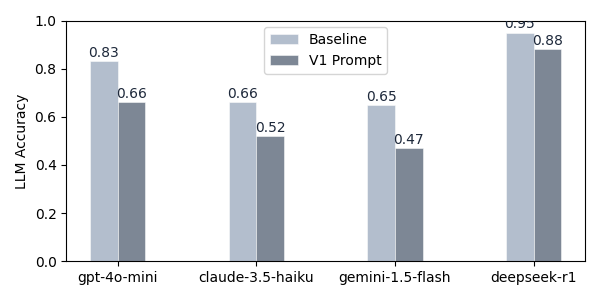
\includegraphics[width=\columnwidth]{images/llm_accuracy_comparison.png}
    \caption{LLM Accuracy Comparison: Baseline vs Enhanced Prompts}
    \label{fig:llm-accuracy}
\end{figure}

Response alignment improved notably with enhanced prompts (Figure \ref{fig:response-alignment}). Claude-3.5-haiku showed the most significant improvement, from 42\% to 69\% alignment, while gpt-4o-mini and gemini-1.5-flash showed modest gains (46\% to 50\% and 32\% to 46\% respectively). This suggests the models better incorporated student context in their decision-making process.

\begin{figure}[H]
    \centering
    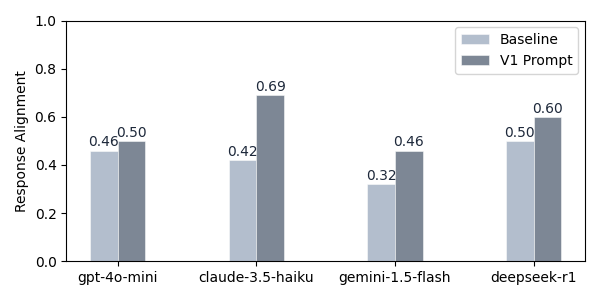
\includegraphics[width=\columnwidth]{images/response_alignment_comparison.png}
    \caption{Response Alignment: Baseline vs Enhanced Prompts}
    \label{fig:response-alignment}
\end{figure}

Exact match rates (Figure \ref{fig:exact-match}) showed smaller improvements, with claude-3.5-haiku achieving the highest gain from 34\% to 44\%, while other models showed minimal changes. This was expected as an exact match is less likely than just correctness alignment, but still represents an improvement compared to the baseline.

\begin{figure}[H]
    \centering
    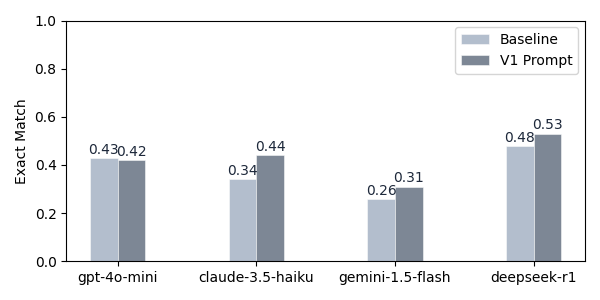
\includegraphics[width=\columnwidth]{images/exact_match_comparison.png}
    \caption{Exact Match Rates: Baseline vs Enhanced Prompts}
    \label{fig:exact-match}
\end{figure}

\subsection{LLM Reasoning Example}

To give a more complete picture of the LLMs' reasoning process, we provide an example of how the LLMs thinks through a given problem and simulate a student's thought process. This example illustrates the LLM's ability to mimic student behavior, including common errors and reasoning patterns.


\begin{questionbox}{Example Question}
    \textbf{Topic:} Multiplication of two-digit numbers \\
    \textbf{Subject:} Natural Numbers \\
    \textbf{Axis:} Arithmetic \\
    
    \textbf{Question:} What is the result of $31 \cdot 12$? \\
    
    \textbf{Options:}
    \begin{itemize}
        \item[(a)] 360
        \item[(b)] 651
        \item[(c)] 93
        \item[(d)] 372
        \item[(e)] None of the above
    \end{itemize}
    
    \textbf{Correct Answer:} b (not shown to the LLM)\\
    \textbf{Actual Student Answer:} c

\end{questionbox}

\begin{studentbox}{Student Characteristics}
    \begin{tabularx}{\textwidth}{Xr}
        \textbf{Age} & 12 \\
        \textbf{Skill Level} & -2.63 \\
        \textbf{Topic Previous Attempts} & 9 \\
        \textbf{Topic Success Rate} & 55\% \\
        \textbf{Subject Previous Attempts} & 34 \\
        \textbf{Subject Success Rate} & 64\% \\
        \textbf{Axis Previous Attempts} & 34 \\
        \textbf{Axis Success Rate} & 64\% \\
    \end{tabularx}
\end{studentbox}

\begin{llmbox}{Gemini 1.5 Flash Response}
    \textbf{Thinking Process:} Okay, so it's multiplication with two-digit numbers.  I'm not the best at this.  Remember those long multiplication problems we did last month?  Those were tricky, and I always got confused with carrying over numbers. I guess I can try to do it step-by-step. I'll first multiply 1 by 31, which is 31. Then, I'll multiply 2 by 31, but I'm not sure how to do that exactly... maybe it's 62?  Hmm, I think it's 62. Now I have to add those two together.  But how do I add them? It's like adding 31 and 62. Maybe the answer is around 90 or something? I see a lot of options, maybe 93? But I'm not sure.  I think it's 93, but I'm not completely sure.  I'm not very good at multiplying two-digit numbers, so I'm probably wrong.
    
    \textbf{Response:} c
    
    \textbf{Confidence:} 60
\end{llmbox}

The LLM is able to personify the student effectively. Given that the student's skill level is fairly low (-2.63), the LLM reasons through the mindset of a student at that level. Despite the question being relatively simple for an LLM, it not only gets the answer wrong but also likely falls for the same distractor option as a student with similar abilities. This demonstrates the LLM's capability to simulate realistic student behavior, including common errors and misconceptions.

\subsection{Preliminary Conclusions}
The results suggest that providing academic context helps LLMs better simulate student behavior by considering ability levels and typical misconceptions. However, these findings are based on a limited sample size. Further research should include:
\begin{itemize}
    \item Conducting studies with larger sample sizes and more repetitions to ensure the reliability and generalizability of the findings.
    \item Incorporating a wider range of student profiles and question types to better understand the LLM's adaptability across diverse scenarios.
    \item Testing with more advanced LLM models to evaluate improvements in simulating student behavior and handling complex questions.
    \item Performing a detailed analysis of specific error patterns to identify common misconceptions and improve the LLM's accuracy.
    \item Refining the prompt by integrating past questions answered by the same student as context. This could involve using questions from the same topic or employing a similarity score (cosine similarity) to perform a vector search and add relevant questions to the prompt, providing additional useful context to the LLM.
\end{itemize}




%----------------------------------------------------------------------------------------
% REFERENCES
%----------------------------------------------------------------------------------------
\printbibliography % Output the bibliography

%----------------------------------------------------------------------------------------

\end{document}
